
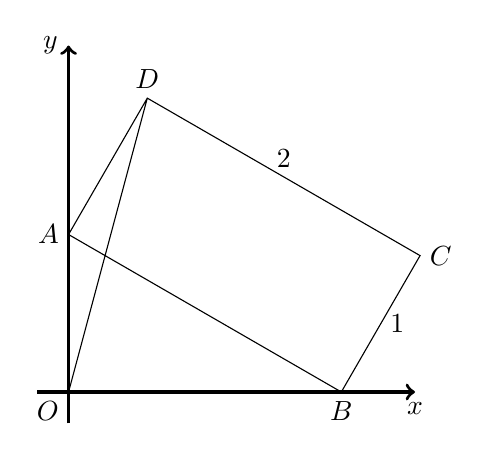
\begin{tikzpicture}[scale=2]
  \coordinate[label=below left:$O$] (O) at (0,0);
  \coordinate[label=left:$A$] (A) at (0,1);
  \coordinate[label=below:$B$] (B) at ({sqrt(3)},0);
  \coordinate[label=above:$D$] (D) at (.5,{1+sqrt(3)/2});
  \coordinate[label=right:$C$] (C) at ({.5+sqrt(3)},{sqrt(3)/2});
  \draw[very thick, ->] (-.2,0) -- (2.2,0) node[below] {$x$};
  \draw[very thick, ->] (0,-.2) -- (0,2.2) node[left] {$y$};
  \draw (A) -- (B) -- node[right] {$1$} (C)
    -- node[above] {$2$} (D) -- cycle (O) -- (D);
\end{tikzpicture}
